\subsection{Wat is een taal?}

\vspace{0.5cm}

\begin{theo}[String over een alfabet $\Sigma$]{String over een alfabet Sigma}
    Een \textbf{string} over een alfabet $\Sigma$ is een eindige opeenvolging van nul, één of meer elementen van $\Sigma$.
\end{theo}

\begin{theo}[Taal $L$ over een alfabet $\Sigma$]{Taal L over een alfabet Sigma}
    Een \textbf{taal} $L$ over een alfabet $\Sigma$ is een verzameling van strings over $\Sigma$.
\end{theo}

\subsection{Een algebra van talen}

\vspace{0.5cm}

\begin{theo}[Een algebra- of algebraïsche structuur]{Een algebra- of algebraïsche structuur}
    Een algebra- of algebraïsche structuur is een verzameling met daarop een aantal inwendige operaties:
    dikwijls binaire operaties, maar unair of met grotere ariteit kan ook. Zo wordt de verzameling van
    alle talen over een alfabet $\Sigma$ een algebra als we als operaties unie, doorsnede, complement, etc.\ definïeren.
    Meer concreet: als $L_1$ en $L_2$ twee talen zijn, dan is
    \begin{itemize}
        \item de unie ervan een taal: $L_1 \cup L_2$
        \item de doorsnede ervan een taal: $L_1 \cap L_2$
        \item het complement ervan een taal: $\overline{L_1}$
    \end{itemize}
\end{theo}

\begin{pro}[Concatenatie van twee talen]{Concatenatie van twee talen}
    Gegeven twee talen $L_1$ en $L_2$ over hetzelfde alfabet $\Sigma$, dan noteren we de concatenatie van
    $L_1$ en $L_2$ als $L_1L_2$ en definïeren we:
    \begin{equation*}
        L_{1}L_{2} = \{ xy | x \in L_1, y \in L_2\}
    \end{equation*}
    \vspace{-0.3cm}
\end{pro}

\begin{pro}[De Kleene ster van een taal]{De Kleene ster van een taa}
    De Kleene ster van een taal wordt gedefinieerd als volgt:
    \begin{equation*}
        L^* = \cup_{n \geq 0}L^n
    \end{equation*}
    \vspace{-0.5cm}
\end{pro}

\newpage

\subsection{Reguliere expressies en reguliere talen}

\vspace{0.5cm}

\begin{theo}[Reguliere Expressie (RE) over een alfabet $\Sigma$]{Reguliere Expressie (RE) over een alfabet Sigma}
    E is een \textbf{reguliere expressie} over een alfabet $\Sigma$ indien E van de vorm is
    \begin{itemize}
        \item $\epsilon$
        \item $\phi$
        \item $a$ waarbij $a \in \Sigma$
        \item ($E_{1}E_{2}$) waarbij $E_1$ en $E_2$ reguliere expressies zijn over $\Sigma$
        \item ($E_{1}^*$) waarbij $E_1$ een reguliere expressies is over $\Sigma$
        \item ($E_{1}|E_{2}$) waarbij $E_1$ en $E_2$ reguliere expressies zijn over $\Sigma$
    \end{itemize}
    \vspace{-0.3cm}
\end{theo}

\begin{theo}[Reguliere taal]{Reguliere taal}
    Een reguliere expressie $E$ bepaalt een \textbf{reguliere taal} $L_E$ over hetzelfde alfabet $\Sigma$ als volgt:
    \begin{itemize}
        \item als $E = a \ (\text{met} \ a \in \Sigma)$ dan is $L_E = \{a\}$
        \item als $E = \epsilon$ dan is $L_E = \{\epsilon\}$
        \item als $E = \phi$ dan is $L_E = \emptyset$
        \item als $E = (E_{1}E_{2})$ dan $L_E = L_{E_1}L_{E_2}$
        \item als $E = {(E_{1})}^{*}$ dan $L_E = L_{E_1}^*$
        \item als $E = (E_{1}|E_{2})$ dan $L_E = L_{E_1} \cup L_{E_2}$
    \end{itemize}
    \vspace{-0.3cm}
\end{theo}

\subsection{Eindge toestandsautomaten}

\vspace{0.5cm}

\begin{theo}[Niet-deterministische eindige toestandsautomaat (NFA)]{Niet-deterministische eindige toestandsautomaat}
    Een \textbf{niet-deterministische eindige toestandsautomaat} is een 5-tal $(Q,\Sigma, \delta, q_s, F)$ waarbij

    \vspace{0.5cm}

    \begin{minipage}{.56\textwidth}
        \begin{itemize}
            \item $Q$ een eindige verzameling toestanden is
            \item $\Sigma$ is een eindig alfabet
            \item $\delta$ is de overgangsrelatie van de automaat
            \item $q_s$ is de starttoestand
            \item $F \subset Q$ is de verzameling eindtoestanden
        \end{itemize}
    \end{minipage}
    \begin{minipage}{.4\textwidth}
        \begin{center}
            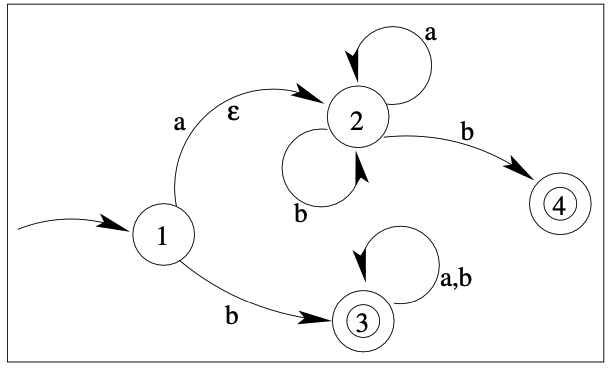
\includegraphics[scale = 0.275]{Images/NFA}
        \end{center}
    \end{minipage}
\end{theo}

\newpage

\begin{theo}[Een string $s$ wordt aanvaard door een NFA]{Een string s wordt aanvaard door een NFA}
    Een string $s$ wordt aanvaard door een NFA $(Q,\Sigma, \delta, q_s, F)$ indien
    er een sequentie $q_s = q_0 \overset{a_0}{\to} \ldots \overset{a_{n-1}}{\to} q_n$
    van overgangen bestaat met $q_n \in F$ zodat s de $\epsilon$-compressiew, wat bekomen wordt door
    in $\epsilon$ te schrappen in de string, is van $a_0 \ldots a_{n-1}$. \\
    
    \noindent \textbf{Dus:} Voor toestanden $p$,$q$ en string $w \in \Sigma^*$ schrijven we $p \overset{w}{\rightsquigarrow} q$
    indien er een sequentie van overangen $ p \overset{a_0}{\to} \ldots \overset{a_{n-1}}{\to} q$ bestaat zodat $w$
    de $\epsilon$-comprssie is van $a_0 \ldots a_{n-1}$.
\end{theo}

\begin{theo}[De taal door een NFA $M$ bepaald]{De taal door een NFA M bepaald}
    Een taal $L$ wordt bepaald door een NFA $M$, indien $L$ de verzameling van strings is die $M$ aanvaardt.
    We noteren de taal van $M$ als $L_M$.
\end{theo}

\begin{theo}[Equivalentie van twee NFA's]{Equivalentie van twee NFA's}
    Twee NFA's worden \textbf{equivalent} genoemd als ze dezelfde taal bepalen.
\end{theo}

\subsection{De algebra van NFA's}

\vspace{0.5cm}

\begin{pro}[De unie van twee NFA's]{De unie van twee NFA's}
    \underline{Gegeven}: ${NFA}_1 = (Q_1,\Sigma, \delta_1, q_{s_1}, \{q_{f_1}\})$ en ${NFA}_2 = (Q_2,\Sigma, \delta_2, q_{s_2}, \{q_{f_2}\})$ \\

    \begin{minipage}{.63\textwidth}
        De unie ${NFA}_1 \cup {NFA}_2$ is de $NFA = (Q,\Sigma, \delta, q_s, F)$ waarbij

        \begin{itemize}
            \item $Q = Q_1 \cup Q_2 \cup \{ q_s, q_f \}$
            \item $F = \{q_f\}$
            \item $\delta$ is gedefnieerd als:
            \begin{itemize}
                \item $\forall q \in Q_{i} \backslash \{q_{f_{i}}\}, \ x \in \Sigma_{\epsilon}, \ i = 1,2: \ \delta(q,x) = \delta_i(q,x)$
                \item $\delta(q_s, \epsilon) = \{q_{s_{1}}, q_{s_{2}}\}$
                \item $\forall x \in \Sigma: \delta(q_s, x) = \emptyset$
                \item $i = 1,2: \delta(q_{f_{i}}, \epsilon) = \{q_f\}$
                \item $\forall x \in \Sigma, i = 1,2: \delta(q_{f_{i}}, x) = \emptyset$
            \end{itemize}
        \end{itemize}
    \end{minipage}
    \begin{minipage}{.33\textwidth}
        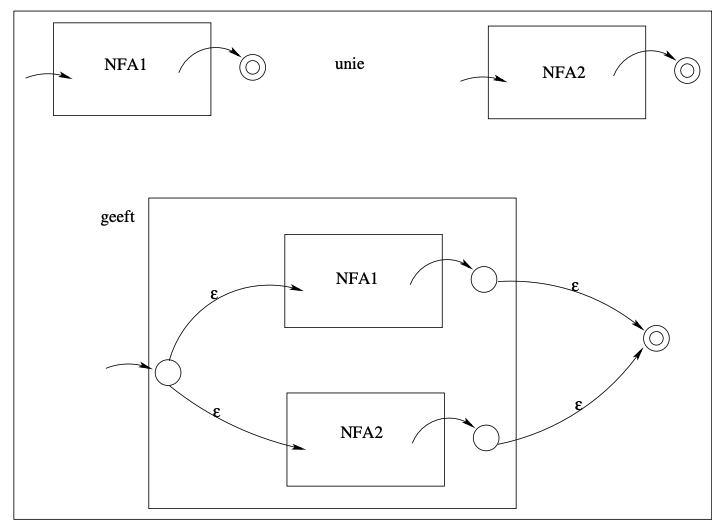
\includegraphics[scale = 0.225]{Images/UnieNFA}
    \end{minipage}
\end{pro}

\newpage

\begin{pro}[De concatenatie van twee NFA's]{De concatenatie van twee NFA's}
    \begin{center}
        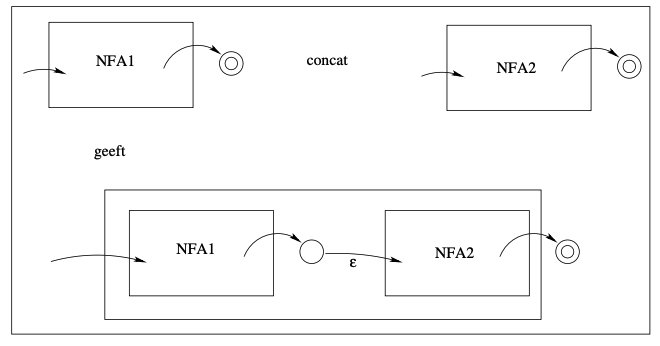
\includegraphics[scale = 0.35]{Images/ConcatNFA}
    \end{center}
\end{pro}

\begin{pro}[De ster van een NFA]{De ster van een NFA}
    \begin{center}
        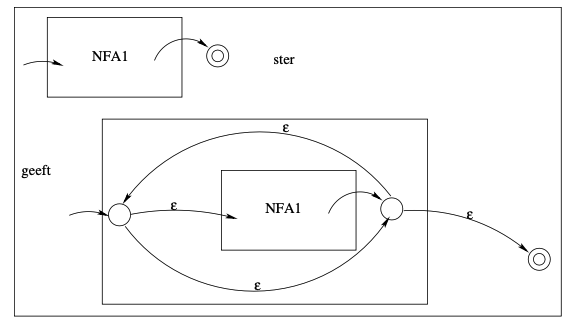
\includegraphics[scale = 0.4]{Images/SterNFA}
    \end{center}
\end{pro}

\subsection{Van RE naar NFA}

\vspace{0.5cm}